\section{Introduction}
Computer aided evolution is becoming increasingly popular for tasks which
involve creating models which have been optimized for certain characteristica.

In general computer evolution approaches the task of evolving candidates
following a Darwinistic approach with populations, selection and
evaluation\cite{paper:ev3}.

Ultimately the goal with such evolution in our case is to develop candidates
which are not the most obvious design choices from a human perspective, but
score a higher grade compared to already known solutions.

An example of such results are space antennas developed by
Hornby\cite{paper:ev4} using generative Computer-Automated Evolutionary
Design[See figure \ref{fig:nasa_antenna}], which have rather controversal
designs. While most antennas are somewhat straight in a direction these
particular antennas are revolving around themselves in arbitrary directions.

\begin{figure}[ht]
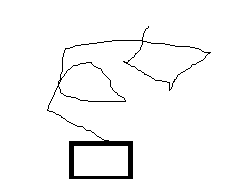
\includegraphics[scale=.7]{content/img/space_antenna}
\caption{Image of the NASA Antenna \cite{paper:ev4} }
\label{fig:nasa_antenna}
\end{figure}

Building from such previous experiences, that something which usually has a
standardized morphology can get so fundamentally different results when applying
EAs, leads us to wanting to apply such methodology to other domains.

The chosen domain is within furniture, namely the types which should be suited
for seating.

One might wonder why this is relevant in current time or in the future? By being
able to produce solutions which are outside of traditional design norms some of
the problems in modern society can be dealt with, problems such as high resource
consumption and strain on the environment when treating the resources.

Since there is a finite amount of raw materials and treatment of aforementioned
resources in the general case results in strain on the environment be it
foraging for wood or producing plastic this project is highly relevant.

%This project focusses on using computer aided evolution to generate models for
%furniture, particularly for the activity of sitting.

By tweaking the parameters to optimize for material or comfort, the candidate
solutions might provide some very interesting and hopefully 'revolutionizing'
designs. Designs which ultimately might save the world.
